\documentclass[12pt]{article}
\usepackage{amsmath}
%\usepackage{fullpage}
\usepackage[top=1in, bottom=1in, left=0.8in, right=1in]{geometry}
\usepackage{multicol}
\usepackage{wrapfig}
\usepackage{graphicx}
\usepackage{float}
\usepackage{listings}
\usepackage{enumerate}
\lstset{language=Java,
	basicstyle={\small\ttfamily},
	columns=flexible,
	belowskip=0mm}

\setlength{\columnsep}{0.1pc}

\title{ME573 Homework Set \# 10}
\author{Alexander Swenson -- \texttt{aaswenson@wisc.edu}}
\date{\today}
\begin{document}
	
	\maketitle
	
	\vspace{-0.3in}
	\noindent
	\rule{\linewidth}{0.4pt}
	
	\noindent
	

\section{Problem 1}
	
	\begin{figure}[!htb]
		\centering
		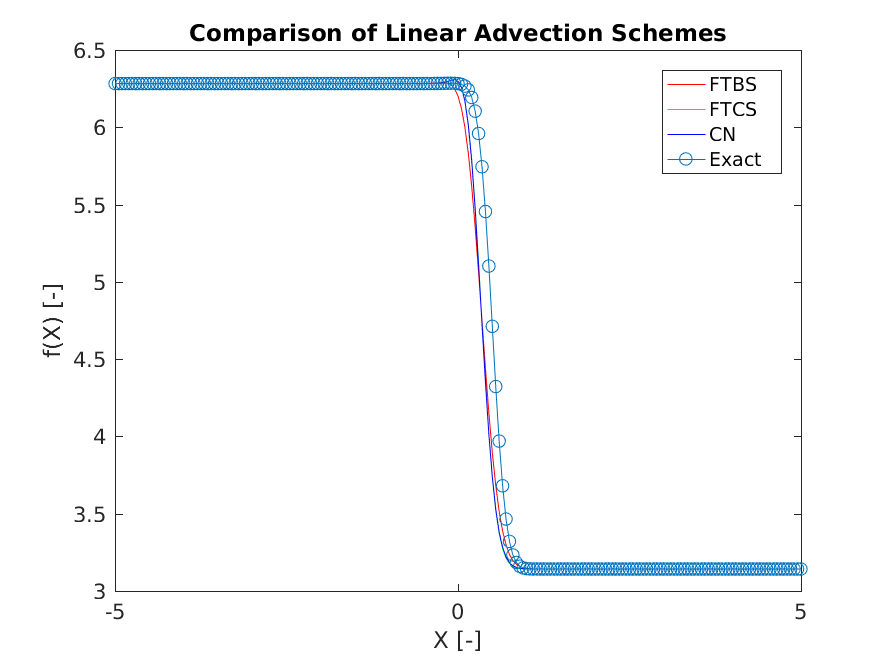
\includegraphics[scale=0.75]{problem1.png}
	\end{figure}

\newpage
\section{Problem 2}
	
	\begin{figure}[!htb]
		\centering
		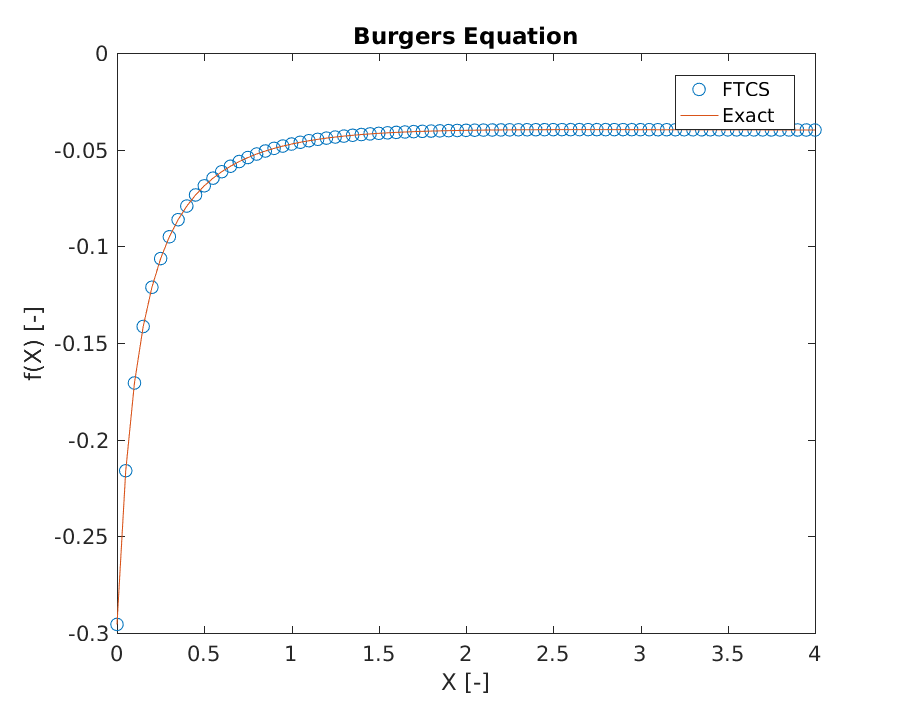
\includegraphics[scale=0.75]{problem2_ftcs.png}
	\end{figure}

	\begin{figure}[!htb]
		\centering
		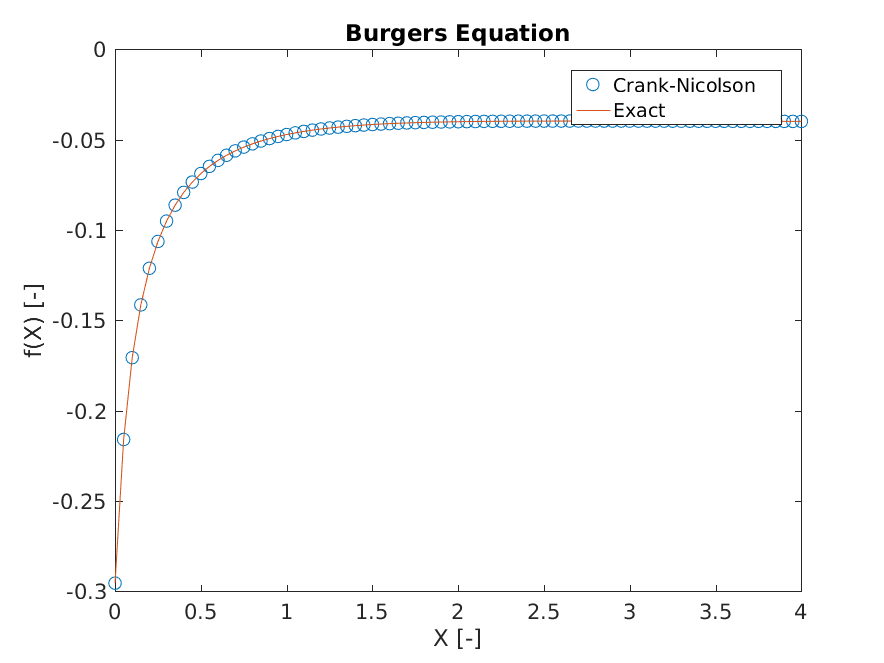
\includegraphics[scale=0.75]{problem2_CN.png}
	\end{figure}




%%%%%%%%%%%%%%%%%%%%%%%%%%%%%%%%%%%%%%%%%%%%%%%%%%%%%%%%%%%%%%%%%%%%%%%%%%%%%%%%

		
	
	
	
	
\end{document}
